\chapter{Stationary properties} 
\label{chap:stationary}
\label{chap:stationary_properties}
The stationary properties of the system are defined by its spectrum. In this chapter the boundary condition is introduced, wavefunctions of the homogeneous wires are obtained, subgap states are investigated and  and the stationary supercurrent is estimated.

\section{Boundary condition}

To obtain the spectrum of the system it's necessary to find the boundary conditions. As the barrier chemical potential  is the biggest energy parameter of the problem, the wave-functions there are defined by the Hamiltonian:
\begin{gather}
\label{barrier_Hamiltonian}
	H(y)
	=
	\br{
		\frac{p^2}{2m}
		+\mu_b
	}\tau_z,  ~~~~~~~~~-\frac{L}{2}<y<\frac{L}{2}.
\end{gather} 

As low energies are the under consideration, in Schroedinger equation the energy term can be omitted, so $ p_b\approx\pm i \sqrt{2m\mu_b} $. One can solve the problem given by (\ref{barrier_Hamiltonian}) and match the values of the wavefunction and its derivatives on the left and on the right of the barrier to obtain:
\begin{gather}
\label{bc_initial}
	\begin{cases}
	\psi_L + b\partial_y\psi_L=t(\psi_R + b\partial_y\psi_R) \\
	\psi_R - b\partial_y\psi_R=t(\psi_L - b\partial_y\psi_L)
	\end{cases}
\end{gather}

here $ \psi_{L,R}=\psi\br{\mp\frac{L}{2}} $, $ b=\br{{2m\mu_b}}^{-\frac{1}{2}} $ --- the penetration depth for the particle inside the barrier and $ t = e^{-\frac{L}{b} }$ --- the tunneling constant assumed to be small: $ t\ll 1 $. This condition means, that the size of the barrier $ L $ should be  much bigger that the penetration depth $ b $.

The condition (\ref{bc_initial}) is invariant under the combined action $ L\leftrightarrow R $, $ y\to-y $. To simplify the further analysis one can reverse the direction in the left wire and shift both ends of the wires from $ y= \frac{L}{2} $ to $ y=0 $. The boundary condition than becomes:
\begin{gather}
\label{bc_transformed}
\begin{cases}
\psi_L - b\partial_y\psi_L=t(\psi_R + b\partial_y\psi_R) \\
\psi_R - b\partial_y\psi_R=t(\psi_L + b\partial_y\psi_L)
\end{cases}
\end{gather}
This transformation is illustrated on the fig \ref{fig:bctransform}. Note

The boundary condition (\ref{bc_transformed}) can be rewritten with the spinor $ \Psi=\br{\psi_L, \psi_R}^T $ and Pauli matrices $ \hat{s}_i $ in LR space:
\begin{gather}
	\br{1-t\hat{s}_x}\Psi-\br{1+t \hat{s}_x}b\pdy\psi=0
\end{gather}
since for all $ t\ne 1 $ (recall, that $ t\ll1 $) the matrix is $ 1\pm t\hat{s}_x $ in invertible Multiplying the last equation by $ \br{1-t\hat{s}_x}/\br{1+t^2} $ obtain:
\begin{gather}
\label{bc_LR_space}
	\br{1-2\tilde{t}\hat{s}_z-\tilde{b}\pdy}\Psi=0
\end{gather}
where $ \tilde{t}=\frac{t}{1+t^2} $, $ \tilde{b} = \frac{1-t^2}{1+t^2}b $. In the leading order in $ t $, which corresponds to the tunneling limit, $ \tilde{t}=t $, $ \tilde{b} = b $.
\begin{figure}[H]
	\centering
	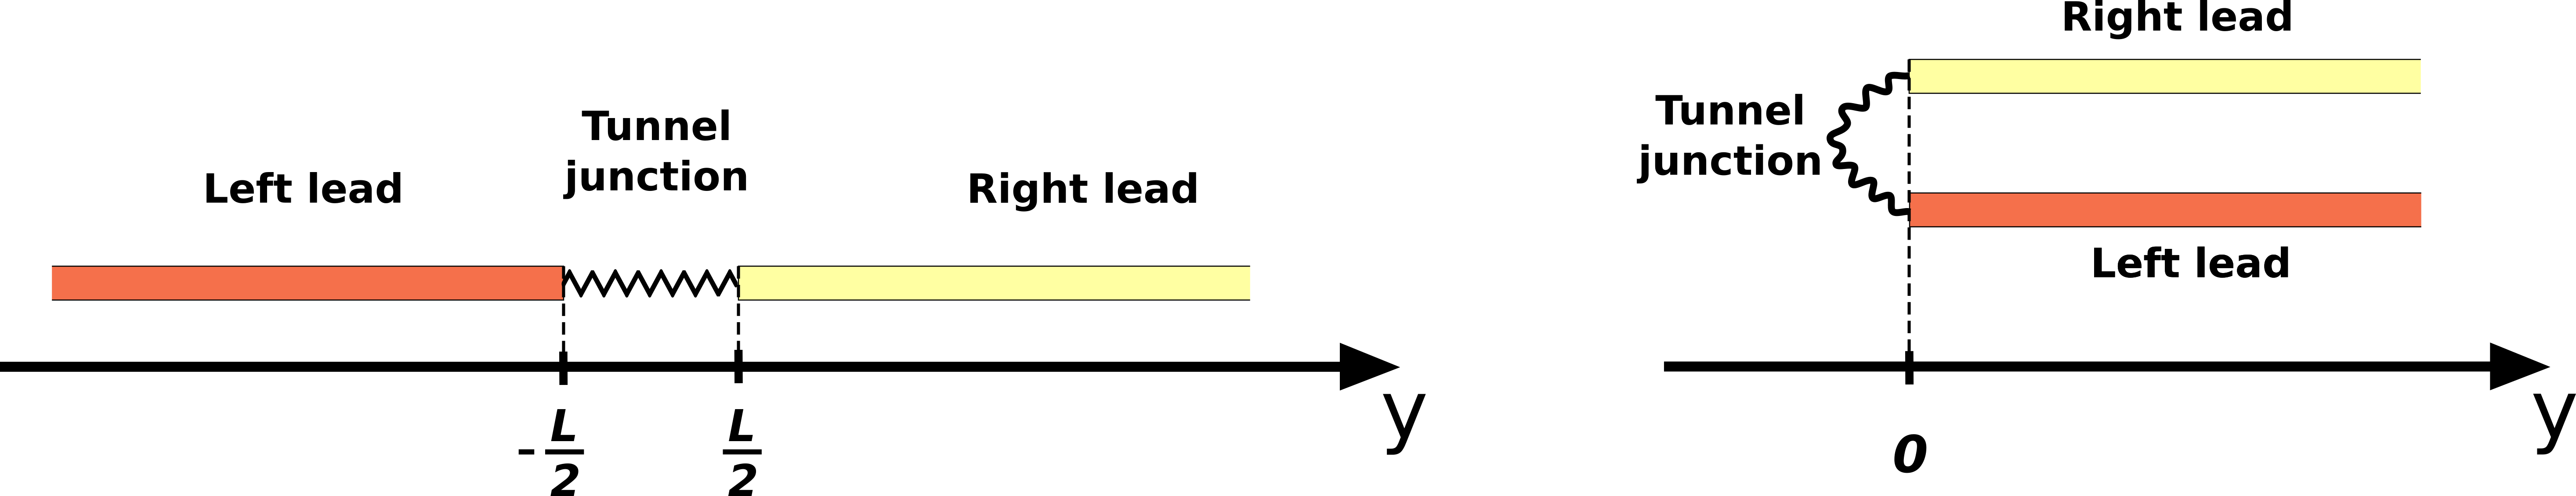
\includegraphics[width=0.9\linewidth]{images/bc_transform}
	\caption{Illustration of switching the direction of left wire}
	\label{fig:bctransform}
\end{figure}

One can argue that in tunneling limit the second and the third term in (\ref{bc_LR_space}) are much smaller than the first one and should not be taken when the leading order is considered. However, if the second terms is omitted, the leads become efficiently disconnected, and no tunnel effects can be found. The same is true for the third term --- if it's not present, the boundary condition immediately implies $ \Psi\br{0} = 0 $, so the wires become disconnected again.

\section{High momentum modes}  

As was pointed in section \ref{sec:high_and_low_modes}, there are  short-wave and long-wave wavefunctions inside the wire, and the former ones can be described with the Hamiltonian (\ref{short-long_hamiltonian}). However, if one is looking for the localized states, even the short-wave modes should be taken decaying. To obtain this, one needs to restore superconducting term in (\ref{short-long_hamiltonian}), so the spectrum become gapped and the momenta get an imaginary part. So, for short-wave modes one should consider an approximate Hamiltonian:
\begin{gather}
\label{high_mods_hamiltonian}
	H=\br{\frac{p^2}{2m}-up\hat{s}_z\sigma_z}\tau_z+\Delta\tau_\phi
\end{gather}
here the multiplier $ \hat{s}_z $ is added in the spin-orbit coupling term, as the direction of the left wire is inverted, so to write a correct Hamiltonian for LR space, one needs to change $ p $ to $ -p $ for the left wire --- which is adding $ -\hat{s}_z $ multiplier to each momentum.

Denoting $ \eta = \frac{p^2}{2m}-up\hat{s}_z\sigma_z $, one can rewrite (\ref{high_mods_hamiltonian}) as $ H=\eta\tau_z+\Delta\tau_\phi $. As $ \hat{s}_z\sigma_z $ commutes with $ H $ one can treat it as a number, so the dispersion is $ E^2 =\eta^2+\Delta^2 $ (the number corresponding to eigenstate of $ \hat{s}_z $ will be denoted as $ s_z $ while the number, corresponding to the eigenstate of $ \sigma_z $ will be denoted as $ \varsigma_z $). Thus $ \eta=\pm i\sqrt{\Delta^2-E^2} $, as the case $ \abs{E}<\Delta $ is assumed. For momenta\textbf{} one can write the equation:
\begin{gather}
	p^2-2mu s_z \varsigma_z p - 2m \eta =0
\end{gather}
which for short-wave momenta gives $ p_{short}\approx2 mu s_z \varsigma_z + \frac{\eta}{u}s_z\varsigma_z$. Choosing the sign of $ \eta $ in a way, that the wavefunction decays at $ x\to +\infty $,  obtain:
\begin{gather}
\label{short_momentum_decaying}
	p_{short}\approx
	2 mu s_z \varsigma_z 
	+
	i\frac{\sqrt{\Delta^2-E^2}}{u}
\end{gather}


Now the wavefunction can be constructed by putting (\ref{short_momentum_decaying}) into the Schroedinger equation $ \br{\eta\tau_z +\Delta\tau_\phi}\Psi=E\Psi $. The solutions are:
\begin{gather}
	\Psi_{s_z,\varsigma_z}\br{x}
	=
	\begin{pmatrix}
	1
	\\
	e^{i\br{s_z\varsigma_z\gamma+\phi_{s_z}}}
	\end{pmatrix}_{eh}
	e^{2imus_z\varsigma_zx -\frac{\sqrt{\Delta^2-E^2}}{u}x}
	\ket{s_z, \varsigma_z}
\end{gather}
where  $ \ket{s_z, \sigma_z} $ are eigenvectors of $ \hat{s}_z \sigma_z $,  $ \gamma = -\frac{\pi}{2}+\arcsin\frac{E}{\Delta} $ and $ \phi_{1}=\phi_L$, $ \phi_{-1}=-\phi_R $
Thus the long-wave part the wavefunction can be written as:
\begin{gather}
\label{fast_mode_expansion}
	\Psi_{long}
	=
	\sum_{s_z=\pm 1}
	\sum_{\varsigma_z=\pm 1}
	C_{s_z,\varsigma_z}
	\Psi_{s_z,\varsigma_z}\br{x}
\end{gather}
 
  \if 0
\begin{gather}
\begin{pmatrix}
i \hat_z \sigma_z\sqrt{\Delta^2-E^2}-E & \Delta e^{-i\phi_{L,R} s_z} \\
\Delta e^{i\phi_{L,R} s_z} & -i s_z \sigma_z\sqrt{\Delta^2-E^2}-E
\end{pmatrix}
\Psi
=
E\Psi
\end{gather}
\fi


\section{Eliminating long-wave modes from boundary condition}
\label{sec:elimintaing_long-wave}
As the Majorana mode acts at low energies, it's expected to be predominantly long-wave. This argument is in accord with \cite{Oreg_2010} and \cite{Lutchyn_2010}, where the Majorana state was an eigenstate of a linearized Hamiltonian, which is relevant only for long-wave physics. So, it's reasonable to eliminate the short-wave modes from the problem, reformulating the boundary condition (\ref{short-long_hamiltonian}).

The wave function can be decomposed in short-wave and  long-wave  parts: $ \Psi = \Psi_{high}+\Psi_{low} $. inserting it into the (\ref{short-long_hamiltonian}) and using the fact, that $ p_{low}\ll p_{high} \approx 2mu s_z \sigma_z $, one can obtain at the boundary:
\begin{gather}
	\br{1-2t\hat{s}_x}\Psi_{low}+\br{1-2t\hat{s}_x-2ibum\hat{s}_z \sigma_z}\Psi_{high}=0
\end{gather}
Multiplying by the $ \br{1-2t\hat{s}_x}^{-1} $ and omitting $ {t^2} $ terms, obtain:
\begin{gather}
	\Psi_{low}
	=
	\br{-1+i\zeta\br{1+2t\hat{s}_x}s_z \sigma_z}\Psi_{high}
\end{gather}
with $ \zeta=2bum $.

Now, using the expansion (\ref{fast_mode_expansion}) and renormalizing the coefficients: $ C_{s_z \varsigma_z}\to-\br{1-i\zeta s_z \varsigma_z}C_{s_z \varsigma_z} $ one can rewrite the boundary condition for $ \varsigma_z $ spin component of the wavefunction as:
\begin{gather}
\Psi_{low,\varsigma_z}
=
\br{1+\frac{2i\zeta t\hat{s}_z\sigma_z}{1+i\zeta \hat{s}_z\sigma_z}}
\sum_{s_z=\pm1}
C_{s_z,\varsigma_z}
		\begin{pmatrix}
	1
	\\
	e^{i\br{s_z\varsigma_z\gamma+\phi_{s_z}}}
	\end{pmatrix}_{eh}
	e^{2imus_z\varsigma_zx -\frac{\sqrt{\Delta^2-E^2}}{u}x}
	\ket{s_z, \varsigma_z}
\end{gather}
This can be  multiplied by $ \br{1+\frac{2i\zeta t\hat{s}_z\sigma_z}{1+i\zeta \hat{s}_z\sigma_z}}^{-1} $, which up to a $ t^2 $ correction yields:

\begin{gather}
\label{bc_projection}
	\br{1-\frac{2i\zeta t\hat{s}_z\sigma_z}{1+i\zeta \hat{s}_z\sigma_z}}
	\Psi_{low,\varsigma_z}
	=
	\sum_{s_z=\pm1}
	C_{s_z,\varsigma_z}
			\begin{pmatrix}
	1
	\\
	e^{i\br{s_z\varsigma_z\gamma+\phi_{s_z}}}
	\end{pmatrix}_{eh}
	e^{2imus_z\varsigma_zx -\frac{\sqrt{\Delta^2-E^2}}{u}x}
	\ket{s_z, \varsigma_z}
\end{gather}

For each $ \varsigma_z $ the above equation can be interpreted as the requirement that the l.h.s. 4-vector (in LR- and eh-spaces) lies in the 2d linear space $ L_{2} $ spanned by the the two vectors in the sum in the r.h.s.. This can be reformulated as the requirement that the l.h.s. be orthogonal to the complementary 2d space $ \overline{L}_{2} $. There are two basic vectors $ \overline{\Psi}_{s_z\varsigma_{z}} $ ($ s_z=\pm1 $) spanning $ \overline{L}_{2} $ for each $ \varsigma_z $:
\begin{gather}
	\overline{\Psi}_{s_z\varsigma_{z}}
	=
	\begin{pmatrix}
	1 \\
	-e^{
		i\br{
			s_z\varsigma_z\gamma
			+
			\phi_{s_z}
			}
		}
	\end{pmatrix}
	\ket{s_z,\varsigma_z}
\end{gather}
Thus one needs to multiply (\ref{bc_projection}) by $ \br{\overline{\Psi}^T_{+\varsigma_{z}},\overline{\Psi}^T_{-\varsigma_{z}}} $ from the left and, after all evaluating the matrix product, find the boundary condition on long-wave modes in the form:
\begin{gather}
\label{bc_matrix}
\begin{pmatrix}1 & -e^{-i\left(\varsigma_{z}\gamma-\phi_L\right)} & A & -Ae^{-i\left(\varsigma_{z}\gamma-\phi_L\right)}\\
A^{*} & -A^{*}e^{i\left(\varsigma_{z}\gamma+\phi_R\right)} & 1 & -e^{i\left(\varsigma_{z}\gamma+\phi_R\right)}
\end{pmatrix}\Psi_{long, \varsigma_{z}}=0
\end{gather}
here $ A=-\frac{2i\zeta t\varsigma_z}{1+i\zeta\varsigma_z} $ and the elements are ordered as $ \br{Le,Lh,Re,Rh} $.

When studying wavefunctions in superconductors, it is more convenient to work with zero phase $ \phi $. This can be achieved by gauging the phase difference into the boundary condition. Indeed, suppose $ H_{\phi} $ describes a wire with phase $ \phi $. Then, $ H_{\phi}=U_{\phi}^{\dagger}H_{0}U_{\phi} $ with $ U_{\phi}=\mathrm{diag(1,e^{i\phi})_{eh}} $ and the wave functions are also related via unitary rotation $ \psi_{\phi}=U_{\phi}^{\dagger}\tilde{\psi} $. So the transform $ U^{\dagger}=\mathrm{diag}\br{1,e^{-i\phi_L},1,e^{-i\phi_R }}_{Le,Lh,Re,Rh}$  will eliminate all the phases from the wires and put them into the boundary condition. Substituting $ \Psi_{low,\varsigma_{z}}=U^{\dagger}\tilde{\Psi} $ into (\ref{bc_matrix}) one arrives at an even simpler boundary condition on the zero-phase function $ \tilde{\Psi} $:
\begin{gather}
\label{bc_matrix_phases}
\begin{pmatrix}1 & -e^{-i\varsigma_{z}\gamma} & A & -Ae^{-i\left(\varsigma_{z}\gamma+\varphi\right)}\\
A^{*} & -A^{*}e^{i\left(\varsigma_{z}\gamma+\varphi\right)} & 1 & -e^{i\varsigma_{z}\gamma}
\end{pmatrix}
\tilde{\Psi}_{long, \varsigma_{z}}=0
\end{gather}
where $ \varphi=\phi_R-\phi_L $. Note, that any physical quantity can depend only on phase difference $ \varphi $,  but not on $ \phi_L $ or $ \phi_R $ separately.

It's also convenient to rewrite it in the form acting on the left and right wire wavefunctions: 

\begin{gather}
\label{bc_matrix_LR}
M_L\tilde{\psi}_{low}^L
+
M_R\tilde{\psi}_{low}^R
=
0
\nonumber
\\
M_L
=
	\begin{pmatrix}
	1 & -e^{-i\sigma_z\gamma}
	\\
	A^* & -A^* e^{i\br{\sigma_z\gamma+\varphi}}
	\end{pmatrix}_{eh}
	\qquad
M_R
=
	\begin{pmatrix}
	A & -A e^{i\br{\sigma_z\gamma+\varphi}}
	\\
1 & -e^{i\sigma_z\gamma}
\end{pmatrix}_{eh}
\qquad	
\end{gather}
This for is especially useful for finding subgap states localized near the barrier.
\section{Low momenta and linearized Hamiltonian}
\label{sec:linearized_hamiltonian}

To utilize boundary condition (\ref{bc_matrix}) or (\ref{bc_matrix_phases}), it's necessary to find low momenta wavefunctions in homogeneous wire (this functions constitute $ \psi_{low}$ in (\ref{bc_matrix}) and (\ref{bc_matrix_phases}). For this purpose one can use the linearized version of the Hamiltonian (\ref{bulk_Hamiltonian}), like in \cite{Oreg_2010} and \cite{Lutchyn_2010}:
\begin{gather}
\label{linearized_hamiltonian}
		H
	=
	-\mu \tau_z
	+
	u p \sigma_z \tau_z
	+
	B\sigma_x	
	+
	\Delta\tau_x
\end{gather}
here zero phase $ \phi $ is assumed and $ \mu $ is equal $ \mu_L $ or $ \mu_R $ depending on the wire considered. As was mentioned before, a nonzero phase can be restored by using $ U_\phi $ matrix. This Hamiltonian is valid only for the right wire. To obtain the solution in the left wire one needs to reverse the sign of $ p $ in (\ref{bulk_Hamiltonian}). Instead of doing so, the unitary transform $ \psi_L=\sigma_x\psi_R $ can be utilized, as $ H\br{-p}=\sigma_x H\br{p}\sigma_x $.

Remembering, that $ \beta=B-\Delta\ll B, \Delta $, one can	treat this Hamiltonian perturbatively and decompose it as $ H=H_0+V_0$:
\begin{gather}
	H_0=
	u p \sigma_z \tau_z
	+
	\Delta
	\br{\sigma_x	
	+
	\tau_x}
\\
V=-\mu \tau_z+\beta\sigma_x
\end{gather}

As $ H_0 $ commutes with $ \sigma_x\tau_x $, it's convenient to rewrite it in the basis of common eigenstates of $ \sigma_x $ and $ \tau_x $. Denoting them as $ \ket{\sigma_x, \tau_x }$ and arranging the order as $  \br{\ket{+, + },\ket{-, - },\ket{+, - },\ket{-, + }} $ one can rewrite $ H_0+V $ as:
\begin{gather}
	H_0
	=
	\begin{pmatrix}
	2\Delta & up & 0 & 0 \\
	up & -2\Delta & 0 & 0\\
	0 & 0 & 0 & up \\
	0 & 0 & up & 0 
	\end{pmatrix},
	~~~~~~~~
	V
	=
		\begin{pmatrix}
	\beta & 0 & -\mu & 0 \\
	0 & -\beta & 0 & -\mu\\
	-\mu & 0 & \beta & 0 \\
	0 & -\mu & 0 & -\beta 
	\end{pmatrix}
\end{gather}
It's easy to see, that the wavefunctions from the subspace $ \mathrm{Span}\br{\ket{+, + },\ket{-, - }} $ require no perturbation to obtain the eigenstates in the leading order. Indeed, diagonalizing the upper subblock of $ H_0 $, one finds, that $ E=\sqrt{\br{2\Delta}^2+\br{up}^2} $. When the low energy states are the objects of interest ($ E\sim g_{L,R} $), one finds, that $ p =\pm\frac{i\Delta}{2u} $ in the leading order, and the corresponding eigenstates are $\ket{+, + }\pm i\ket{-, - } $. 

The another two eigenstates are a little bit more complicated. Diagonalizing  the lower subblock of $ H_0 $, one immediately finds, that $ E=\pm up $. This corresponds to the fact, that $ H_0 $ is the version of $ H $ with a closed gap $ g $  on lower branch (see fig. \ref{fig:spectrum},(e)), so in the zero order these states cannot form anything localized at all. To find them correctly, one needs to take into account the perturbation $ V $ and solve the secular equation using the following ansatz:
\begin{gather}
	\psi = r_1\ket{+, + }+r_2\ket{-, - }+q_{1}\ket{+, - }+q_{2}\ket{-, + }
\end{gather}
with $ r_i\ll q_j $ for all  pairs $ \br{i,j} $. In the leading order (remember, that both $ E  $ and $ up $ are of the order of $ g_{L,R} $ now) this results in a couple of equations:
\begin{gather}
\begin{cases}
	\br{-E+B-\Delta-\frac{\mu^2}{2\Delta}}q_1+up q_2=0
	\\
	u p q_1 + \br{-E-B+\Delta+\frac{\mu^2}{2\Delta}}q_2 =0
\end{cases}
\end{gather}
recall, that $ g=B-\Delta-\frac{\mu^2}{2\Delta} $ and find $ E^2=g^2+u^2p^2 $.

For this states the momenta are of the order of $ g/u $, so it's reasonable to name them long-wave states. Then the states with momenta $ \pm\frac{i\Delta}{2u} $ will be called medium-wave states.

Now it's time to present these wavefunctions in original BdG basis. The expressions here are relevant only for the right wire and for $ E>0 $. To find the wavefunctions in the left wire, the transform $ \psi_L=\sigma_x\psi_R $ is used, while for finding the negative energy states we utilize electron-hole transform: $ \psi_{E<0}= \tau_y\sigma_yK\psi_{E>0}$ with $ K $ being a complex conjugation operator.

For $ E>2\Delta $ medium wave states are:
\begin{gather}
	\psi^{out,~in}_{medium}
	\bigg|_{E>2\Delta}
	=
	\begin{pmatrix}
	1
	\\
	\frac{E\mp\sqrt{E^2-4\Delta^2}}{2\Delta}
	\\
	\frac{E\mp\sqrt{E^2-4\Delta^2}}{2\Delta}
	\\
	1
	\end{pmatrix}
	e^\frac{\pm i x\sqrt{E^2-4\Delta^2}}{u}
	\end{gather}
	
	For $ E>2\Delta $ medium wave states are:
	\begin{gather}
	\label{medium_dec_wave_functions}
	\psi^{grow,~dec}_{medium}
	\bigg|_{E<2\Delta}
	=
	\begin{pmatrix}
	1
	\\
	\frac{E\pm i\sqrt{4\Delta^2-E^2}}{2\Delta}
	\\
	\frac{E\pm i\sqrt{4\Delta^2-E^2}}{2\Delta}
	\\
	1
	\end{pmatrix}
	e^\frac{\pm  x\sqrt{4\Delta^2-E^2}}{u}
\end{gather}

For $ E>\abs{g} $ long-wave states are:
\begin{gather}
		\psi^{out,~in}_{long}
		\bigg|_{E>g}
=
\begin{pmatrix}
1\\
\frac{E\mp \sqrt{E^2-g^2}}{g}\\
-\frac{E\mp \sqrt{E^2-g^2}}{g}\\
-1
\end{pmatrix}
e^{\pm\frac{ix\sqrt{E^2-g^2}}{u}}
\end{gather}
For $ E<\abs{g} $ long-wave states are:
\begin{gather}
	\label{long_dec_wave_functions}
	\psi^{grow,~dec}_{long}
	\bigg|_{E<g}
	=
	\begin{pmatrix}
	1\\
	\frac{E\pm i\sqrt{g^2-E^2}}{g}\\
	-\frac{E\pm i\sqrt{g^2-E^2}}{g}\\
	-1
	\end{pmatrix}
	e^{\pm\frac{x\sqrt{g^2-E^2}}{u}}
\end{gather}

\section{Subgap states}
\label{sec:Subgap_states}

To find the bound states one needs to make two linear combinations (each for it's own wire) of decaying wave functions from (\ref{medium_dec_wave_functions}) and (\ref{long_dec_wave_functions}) at $ x=0 $ and put them into boundary condition (\ref{bc_matrix_LR}). For the right wire they can be taken directly from (\ref{medium_dec_wave_functions}) , (\ref{long_dec_wave_functions}), while for the left wire they should be multiplied by $ \sigma_x $ from the left (see the beginning of section \ref{sec:linearized_hamiltonian}).. These linear combinations can be written as:
\begin{gather}
	\tilde{\psi}_L
	=
	C_{medium}^L
	\sigma_x \psi^{dec}_{medium}
	+
	C_{long}^L
	\sigma_x \psi^{dec}_{L,long}
\qquad
	\tilde{\psi}_R
	=
	C_{medium}^R
	\psi^{dec}_{medium}
	+
	C_{long}^R
	\psi^{dec}_{R,long}
\end{gather}
where $ C_{medium}^L,C_{long}^L, C_{medium}^R,C_{long}^R $ are the undefined coefficients. Note, that the spinor $ \psi^{dec}_{medium} $ is the same for the left and for the right wires.

 Putting these combinations into boundary condition \ref{bc_matrix_LR}, one can obtain four equations for these coefficients. If this system has a solution at energy $ E_0 $, than there is a bound state with this energy. The condition of solvability can be written as:
\begin{gather}
\label{subgap_determinant}
	\det F = 0
\end{gather}
where matrix $ F $ is given by:
\begin{gather}
F
=
	\begin{pmatrix}
	M_L \sigma_x \psi^{dec}_{medium},
	&
	M_L 
	\sigma_x \psi^{dec}_{L,long},
	&
	M_R
	\psi^{dec}_{medium},
	&
	M_R
	\psi^{dec}_{R,long}
	\end{pmatrix}
\end{gather}
As $ E\sim g_{L,R}\ll\Delta $, the medium-wave spinor can be taken in it's low-energy form: 
In the most part of this work the low energy version: $\psi_{medium}^{dec}\approx
\br{
	1,
	- i,
	- i,
	1
}^T
 $
will be used.

For dealing with $ \psi^{dec}_{long} $ it's convenient two introduce to quantities $ \chi_{L,R} $:
\begin{gather}
\cosh\chi_{L,R}
=
\frac{g_{L,R}}{\sqrt{g^2_{L,R}-E^2}}
\qquad
\sinh\chi_{L,R}
=
\frac{E}{\sqrt{g^2_{L,R}-E^2}}
\end{gather}

If $ g>0 $, the corresponding parameter $ \chi $ is real and the monotonously growing with $ E $. For $ g<0 $ the corresponding is complex, but can be parametrized as $ \chi=-\tilde{\chi}+i\pi $ with real and monotonous $\tilde{\chi}  $.

With this parameters the spinors $ \psi_{L\br{R},long}^{dec} $ at $ x=0 $ can be written as:
\begin{gather}
\psi_{L\br{R},long}^{dec}
=
	\begin{pmatrix}
	-\sinh \chi_{L\br{R}} -i
	\\
	-\cosh \chi_{L\br{R}}
	\\
	\cosh \chi_{L\br{R}}
	\\
	\sinh \chi_{L\br{R}} +i
	\end{pmatrix}
\end{gather}
This parametrization completes the toolset used for studying the subgap states.

\subsection{The case of zero tunneling}
\label{subsect:zero_tunnel}
Consider first the the equation (\ref{subgap_determinant}) with $ t=0 $. This corresponds to absolutely unpenetrable barrier, orm which is same, to independent wires ended with a vacuum. The computation of the determinant in (\ref{subgap_determinant}) becomes a rather easy problem and results in:
\begin{gather}
\label{det_bound_States_zero_t}
	\det F
	\Big|_{t=0}
	=
	-16 \left(i \sinh \left(\chi _L\right)+\cosh \left(\chi _L\right)-1\right) \left(i \sinh \left(\chi _R\right)+\cosh \left(\chi _R\right)-1\right)
\end{gather}

If both $ g_L $, $ g_R $ are negative (triv-triv junction), this determinant cannot be equal to zero at all, as $ \cosh \chi_{L,R} $ are also negative and the real part in each braces always non zero.  If one of $ g_L $, $ g_R $ (triv-top junction), say $ g_R $ there is only one solution at $ E=0 $. If there both $ g_L $, $ g_R $(top-top junction) are positive, there are two solutions at $ E=0 $.

This result proves, that the presence of Majorana mode in a isolated wire is defined only by the sign of $ g $ and justifies the notion of  topology in this system.

\subsection{Small tunneling}
To take into account the tunneling effect one may decompose $ \det F $ in $ t $. Note, that there is no first order in $ t $ due to the structure of boundary condition (\ref{bc_matrix_phases}). The decomposition can be written as:
\begin{gather}
\label{det_f_decomposition}
	\det F
	=
	d_0
	+
	d_2t^2
	+
	\dots
\end{gather}
where $ d_0 $ is given by (\ref{det_bound_States_zero_t}). $ d_2 $ can be computed in a same way, but appears to be  a rather complex formula.  However, in tunneling limit the second correction in (\ref{det_f_decomposition}) should be much smaller than the first one, so the only values of $ E $ that should be considered are the ones with $ d_0 $ is close to zero.

For triv-triv junction there are no such points, so in the tunneling limit there are no bound states for this case.

For triv-top junction there is a solution for $ E=0 $, which corresponds to $ \chi_L=i \pi $, $ \chi_R=0 $. Computing $ d_2 $ for this parameters, one finds that it's exactly zero, so there is no correction to Majorana energy --- as at should be, as it's protected by a particle-hole symmetry.

For top-top junction the situation is more interesting. In that case there are two solutions at $ E=0 $, which should split for nonzero $ t $. Calculating $  $ $ d_2 $ at $ E=0 $ and decomposing $ d_0 $ for small $ E $, one finds:
\begin{gather}
d_0=\frac{16E^2}{g_Rg_L}
\qquad\qquad
	d_2 = -\frac{256t^2\zeta^4}{\br{1+\zeta^2}^2}\cos^2\frac{\phi}{2}
\end{gather}
Using, that $ \zeta=2bum\ll1 $, one can find the energy levels:
\begin{gather}
	E_{1,2}
	=
	\pm
	4t\zeta^2\sqrt{g_Rg_L}\cos\frac{\phi}{2}
\end{gather}
this answer is relevant only if these level are well below the gaps: $ t\zeta^2\sqrt{g_Rg_L}\ll\min\left[g_R,g_L\right] $.
\section{Stationary supercurrent }

\label{sec:stationary_supercurrent}
The stationary supercurrent for a Josephson contact is defined by \cite{Beenakker_three_universal}:

\begin{multline}
\label{beenakker_current}
	I =
	-
	\frac{2e}{\hbar}
	\sum_p
	\tanh\br{\frac{\varepsilon_p}{2k_BT}}
	\frac{d \varepsilon_p}{d\varphi}
	-
	\\
	-
	\frac{4e}{\hbar}
k_BT
	\int\limits_{cont.}d\varepsilon \log
	\left[
		2\cosh\br{\frac{\varepsilon}{2k_BT}}
	\right]
	\frac{d\rho}{d\varphi}
	+
	\frac{2e}{\hbar}
	\frac{d}{d\varphi}
	\int
	d y
		\frac{\abs{\Delta}^2}{\abs{ c}}
\end{multline}
Here $ \epsilon_p $ are the energies of the states localized near the barrier, $ \rho$ is the density of states and $ c\br{\textbf{r}} $ is the interaction constant of the BCS theory, $ \varphi $ is a phase difference, $ k_B $ is Boltzmann's constant and $ T $ is the temperature.
The first term comes from the discrete spectrum and the sum is taken over all states in it, the second term is the current from continuous spectra and the third  term comes from inhomogeneity of the order parameter. As pointed in \cite{Beenakker_three_universal}, despite being generally nonzero, this last term doesn't contribute when step-model functions $ \Delta $ like in (\ref{full_hamiltonian_suppl})  are used.

After omitting the third term and taking the low temperature limit one rewrites (\ref{beenakker_current}) as:
\begin{gather}
\label{current_low_T}
		I =
		-
	\frac{2e}{\hbar}
	\sum_p
	\frac{d \varepsilon_p}{d\varphi}
	-
	\frac{2e}{\hbar}
	\int\limits_{cont.}\varepsilon d\varepsilon 
	\frac{d\rho}{d\varphi}
\end{gather}

Here the only unknown quantity  is the density of states. As there is a derivative over $ \phi $ taken, one need to find the phase dependent part of $\rho  $ only. It can be done by using the relation between the density of states and the scattering matrix \cite{Akkermans_Avron_Shapiro_scattering_matrix}:
\begin{gather}
\label{smatrix_and_DOS}
	\rho\br{\phi}=\frac{1}{2\pi i}\frac{\partial}{\partial \varepsilon}\log \det \hat{S} +const.
\end{gather}

As was showed in the section \ref{sec:Subgap_states}, there are no subgap states in triv-top contact except Majorana state. But this state lays exactly on zero energy regardless of the phase difference, so the derivative in the first term of (\ref{current_low_T}) will be zero and no supercurrent from the Majorana state is present.

The scattering matrix can be found with the help of boundary condition (\ref{bc_matrix_phases}) and the results of section (\ref{sec:linearized_hamiltonian}). It's dimension depends of the number of propagating modes at given energy. In this section only the triv.-top. contact will be considered, while the scattering matrices and DOS for other types of contacts will be given in the appendix.

The process of building s-matrix is the following. Firstly, it's necessary to consider an energy and all the propagating  wavefunctions at this energy. Among them there are wave functions, localized near the barrier ($ \mathrm{Im}p>0 $), propagating towards the barrier ($  p<0 $), and propagating from the barrier ($ p<0 $). Let's denote these  three sets as $ X_{local} $, $ X_{in}  $ and $ X_{out} $. Each wavefunction $ \psi_i $ may contribute with it's own coefficient $ C_i $ --- denote the vectors of the coefficients  $ \vec{Y}_{local} $, $ \vec{Y}_{in}  $ and $ \vec{Y}_{out} $ . The s-matrix connects the coefficients from $ \vec{Y}_{in}  $ to $ \vec{Y}_{out} $ in a following way:
\begin{gather}
	\vec{Y}_{out} = \hat{S}\vec{Y}_{in}
\end{gather}
to find a row of $ \hat{S} $, one should be taken equal to unity, than take  the functions from $ X_{local} $, $ X_{out} $ and one chosen function $ \Psi_{in,chosen} $ from $ X_{in} $ and make the linear combination of the form: $\Upsilon =\psi^{in}_{chosen} + c^{out}_1\Psi^{out}_1+c^{out}_2\Psi^{out}_2+...+c^{out}_1\Psi^{out}_1+c^{local}_2]Psi^{local}_2+... $. The one needs to act with the matrix $ \ref{bc_matrix_phases} $ on $ \Upsilon $ and obtain a set of equations for the coefficients $ {c^{in}_i} $ and $ {c^{local}_i} $. This system should be solved,and the resulting coefficients ${c^{in}_i}  $ should form a row in $ \hat{S} $, corresponding to $ \Psi_{in,chosen} $ . To construct the entire matrix $ \hat{S} $, one should repeat this procedure for every function $ \Psi_{in,chosen} $ in $ X_{in} $.

The coefficients of $ \hat{S} $ generally depend on the normalization of the wavefunctions in $ X_{local} $, $ X_{in}  $ and $ X_{out} $. To make the formula (\ref{smatrix_and_DOS}) valid, one must take the functions from $ X_{local} $ normalized to unity and the functions from $ X_{in}  $, $ X_{out}$ normalized to a flux\cite{Akkermans_Avron_Shapiro_scattering_matrix}: $ \bra{\psi_{in,out}}v \ket{\psi_{in,out}} $ with $ v $ for our problem being $ v=u\sigma_z\tau_z $.

Here some additional parameters will be used. When the given wavefunction is localized ($ e<g $), $ \theta $-parametrization is used:

\begin{gather}
\theta_{L,R}:~~~\sin \theta_{L,R} =\frac{E}{g_{L,R}},~~~\cos \theta_{L,R}>0
\end{gather}
this parametrization is useful for both trivial and topological wires. When the wavefunction propagates ($ E>g $), the $ \eta $- or $ \kappa $-parametrization is used, depending on the sign of $ g $:
\begin{gather}
	\eta_R: ~~~\cosh\eta_R = \frac{E}{g_R},~~~\sinh \eta_R >0
	~~~~~~~~
	\kappa_L: ~~~ \cosh\kappa_L= \frac{E}{\abs{g_{L}}},~~~\sinh \kappa_L>0
\end{gather}
The way to memorize it is that the $ \eta $ is used for a topological wire, whether the $ \kappa $ is used for a trivial wire. All the parameters $ \theta_{L,R}  $,  $\kappa_L $ and $ \eta_R $ are always real and positive when used.

As the dimension of  s-matrix depends on the number of propagating modes, and thus on the energy, it's necessary to investigate different energy ranges separately.

For $ E\ll\Delta $  one may use low energy limit of functions $ \psi_{medium}^{dec} $: $ \psi_{medium}^{dec}\approx\br{1,-i,-i,1}^Te^{-{\frac{2\Delta x}{u}} }$ and also set $ \gamma=-\frac{\pi}{2}\arcsin\frac{E}{\Delta} \approx -\frac{\pi}{2}$. When $ E\sim\Delta $ one has to use $ \gamma $ as it is, and high energy of $ \psi_{low}^{dec} $: $  \psi_{low}^{dec}\approx\br{1,0,0,1}e^{-\frac{Ex}{u}}$.

\subsection{$ E $ \hspace{0pt} between $ \abs{g_L} $ and $ g_R $}

Also recall, that the trivial wire is placed on the left of the barrier while the topological wire is on the right of it. There are two slightly distinct cases, which differ by relation between $ g_L $ and $ g_R $. 
\subsubsection{The case $ \abs{g_L} > g_R $}

For $ g_R<E<\abs{g_L} $ there is only one state in $ X_{in} $, so the s-matrix has the dimension 1, so it's determinant coincides with it's only matrix element, which reads:
\begin{gather}
	\det \hat{S}
	=
	-\frac{e^{\eta _R}+i}{1+i e^{\eta _R}}-\frac{2 i \zeta ^4 t^2 e^{-i \varphi } \left(1+e^{i \varphi }\right)^2 \left(-1+e^{i \theta _L}\right) \left(e^{2 \eta _R}-1\right)}{\left(\zeta ^2+1\right)^2 \left(1+e^{i \theta _L}\right) \left(e^{\eta _R}-i\right){}^2}+O\left(t^3\right)
\end{gather}

Using the (\ref{current_low_T}) (\ref{smatrix_and_DOS}), one finds, that:
\begin{gather}
\label{curr_e_between_g_r>g_l}
	I=\frac{2e}{\hbar}\frac{4t^2\zeta^4\sin\varphi}{\pi}\br{
		\sqrt{g_L^2-g_R^2}
		-
		\int_{g_R}^{\abs{g_L}}	dE\frac{\sqrt{E^2-g_R^2}}{ \sqrt{1-\frac{E^2}{g_L^2}}+1}}
\end{gather}
\subsubsection{The case $ \abs{g_L} < g_R $}
When $ \abs{g_L}<E<g_R $ there is also only one state in $ X_{in} $ and the s-matrix is:
\begin{gather}
\det\hat{S}
=
	\frac{e^{\kappa _L}-i}{-1+i e^{\kappa _L}}-\frac{2 i \zeta ^4 t^2 e^{-i \varphi } \left(1+e^{i \varphi }\right)^2 \left(e^{2 \kappa _L}-1\right) \left(1+e^{i \theta _R}\right)}{\left(\zeta ^2+1\right)^2 \left(e^{\kappa _L}+i\right){}^2 \left(-1+e^{i \theta _R}\right)}+O\left(t^3\right)
\end{gather}
Again with the help of (\ref{current_low_T}) (\ref{smatrix_and_DOS}), one finds, that:
\begin{gather}
\label{curr_e_between_g_r<g_l}
I=\frac{2e}{\hbar}\frac{4t^2\zeta^4\sin\varphi}{\pi}\br{
	\sqrt{g_R^2-g_L^2}
	-
	g_R
	\int_{\abs{g_L}}^{g_R}
	\frac{dE}{E^2}
	\sqrt{E^2-g_L^2} \left(\sqrt{1-\frac{E^2}{g_R^2}}+1\right)
}
\end{gather}

\subsection{$ E $ \hspace{0pt} is greater than both $ \abs{g_L} $ and $ g_R $ and much smaller than $ \Delta $}

Here there are two states in $ X_{in} $ -- one in the right wire and one in the left, so the s-matrix has the dimension equal to two. Arranging it's elements in the following order:
\begin{gather}
\label{s_matrix_2D}
	\hat{S}
	=
	\begin{pmatrix}
	r_{LL} & t_{LR} \\ 
	t_{RL} & r_{RR}
	\end{pmatrix}
\end{gather}
one gets:

\begin{gather}
	r_{LL}
	=
	\frac{e^{\kappa _L}-i}{-1+i e^{\kappa _L}}+\frac{2 \zeta ^4 t^2 e^{-i \varphi } \left(1+e^{i \varphi }\right)^2 \left(e^{2 \kappa _L}-1\right) \left(e^{\eta _R}+i\right)}{\left(\zeta ^2+1\right)^2 \left(e^{\kappa _L}+i\right){}^2 \left(-1-i e^{\eta _R}\right)}+O\left(t^3\right)
	\\
	r_{RR}
	=
	-\frac{e^{\eta _R}+i}{1+i e^{\eta _R}}
	+
	\frac{2 \zeta ^4 t^2 e^{-i \varphi } \left(1+e^{i \varphi }\right)^2 \left(e^{\kappa _L}-i\right) \left(e^{2 \eta _R}-1\right)}{\left(\zeta ^2+1\right)^2 \left(-1+i e^{\kappa _L}\right) \left(e^{\eta _R}-i\right){}^2}+O\left(t^3\right)
	\\
	t_{LR}=
	\frac{2 \zeta ^2 t e^{-i \varphi } \left(1+e^{i \varphi }\right) \sqrt{\left(e^{2 \kappa _L}-1\right) \left(e^{2 \eta _R}-1\right)}}{\left(\zeta ^2+1\right) \left(e^{\kappa _L}+i\right) \left(e^{\eta _R}-i\right)}+O\left(t^3\right)
	\\
	t_{RL}
	=
	-\frac{2 t \zeta ^2 \left(1+e^{i \varphi }\right) \sqrt{\left(e^{2 \kappa _L}-1\right) \left(e^{2 \eta _R}-1\right)}}{\left(\zeta ^2+1\right) \left(e^{\kappa _L}+i\right) \left(e^{\eta _R}-i\right)}+O\left(t^3\right)
\end{gather}
The computation of supercurrent is again made with the (\ref{current_low_T}) (\ref{smatrix_and_DOS}). Introducing $  $: 
\begin{gather}
	g_{max}
	=
	\begin{cases}
	g_R, ~~g_R>\abs{g_L}
	\\
	g_L, ~~\abs{g_L}>g_R
	\end{cases}
	\qquad
		g_{min}
	=
	\begin{cases}
	g_R, ~~g_R<\abs{g_L}
	\\
	g_L, ~~\abs{g_L}<g_R
	\end{cases}
	\qquad
	s_g
	=
	\begin{cases}
	1,~~g_R>\abs{g_L}
	\\
	-1,~~g_R<\abs{g_L}
	\end{cases}
\end{gather}
one finds:
\begin{multline}
\label{curr_e>g_max}
I\sim
	\frac{2e}{\hbar}\frac{4t^2\zeta^4\sin\varphi}{\pi}\times
	\\
	\times
	\br{
	s_g\sqrt{g_{max}^2-g_{min}^2}
-
g_{max}g_{min}
\int_{g_{max}}^{\Delta}
\frac{dE}{E^2}
\br{
	\frac{\sqrt{E^2-g_{max}^2}}{g_{max}}
	+
	\frac{\sqrt{E^2-g_{min}^2}}{g_{min}}
}
	}
\end{multline}
it's important to note, that this computation is irrelevant for $ E\sim\Delta $, so $ \Delta $ here acts like hight energy cutoff. 

\subsection{$ E $ is near and below $ \Delta $}

To maker the estimate for the supercurrent at energies $ E\lesssim \Delta$ high energy versions of $ \psi_{low} $ can be used, so the system forgets about $ g_L $ and $ g_R $ and becomes effectively symmetric. Taking the notation from (\ref{s_matrix_2D}), find:
\begin{multline}
	r_{LL}=r_{RR}
	=
	e^{i \gamma }+
	\\
	+
	\zeta ^2 t^2 e^{-i \varphi } \left(\frac{\left(-1+e^{2 i \gamma }\right)^2 \left(1+e^{i \varphi }\right)^2}{e^{i \theta }-e^{i \gamma }}+2 e^{i \gamma } \left(e^{2 i (\gamma +\varphi )}+e^{2 i \gamma }-2 e^{i \varphi }\right)\right)
	+O\br{t^3}
	\end{multline}
\begin{gather}
	t_{RL}=-t_{RL}
	=
	i \zeta  t\left(1+e^{2 i \gamma }\right)  \left(-1+e^{i \varphi }\right)
	+
	O\br{t^3}
\end{gather}
Using (\ref{current_low_T}) (\ref{smatrix_and_DOS}), one may find
(\ref{current_low_T}) (\ref{smatrix_and_DOS})
\begin{gather}
\label{curr_E_delta}
I
\sim
	\frac{e}{\hbar}
	\zeta ^2 t^2\Delta
\end{gather}

\subsection{Analyzing the results}
From (\ref{curr_e_between_g_r<g_l}) and (\ref{curr_e_between_g_r>g_l}) one may see, that the current coming from the states between $ g_L $ and $ g_R $ has a multiplier of the order $ g_{L,R} $. The current from the states above $ g_{max} $, but close to it, can be estimated with (\ref{curr_e>g_max}). It has the multiplier $ g_{min}\log\frac{\Delta}{g_{max}} $. The current states near $ \Delta $ according to (\ref{curr_E_delta}) is proportional to $ \Delta $. Thus one may deduce that the current from the low energy states is negligible compared with the current from the states near $ \Delta. $ 

This is similar to the result of short Josephson junction with some bound state below the gap. It can be shown, that in that case the current from the subgap state will be proportional to the same quantity as (\ref{curr_E_delta}).
	

